\chapter{Cadre general du projet}

\section{Introduction}
Avant de presenter les artefacts techniques de Nova~AI, il convient de
decrire le cadre dans lequel le projet s'inscrit. Ce premier chapitre est
donc essentiellement contextuel. Nous commencons par presenter l'organisme
d'accueil dans lequel le projet a pris forme, puis nous elargissons la
perspective au paysage des PME tunisiennes qui a motive le travail. Une
analyse critique des modes de communication existants permettra de poser la
problematique en termes concrets. De la problematique decoulera la solution
proposee --- la plateforme elle-meme --- et nous cloturons le chapitre par
la methodologie de gestion de projet (Agile Scrum) adoptee pour la
realisation iterative.

\section{Presentation de l'organisme d'accueil}

\subsection{Bref historique}
\textit{[Remplacer ce paragraphe par l'historique reel de votre organisme
d'accueil : date de fondation, marches geographiques desservis, jalons
notables, mission. Si Nova~AI a ete realise comme un projet entrepreneurial
personnel plutot qu'au sein d'une entreprise, remplacer cette section par une
description du marche cible : le paysage des PME tunisiennes, la penetration
de WhatsApp dans le pays, et le contexte reglementaire pertinent.]}

A titre d'exemple a remplacer : \og [Nom de l'entreprise] est une societe
tunisienne de developpement logiciel fondee en [annee], specialisee dans la
realisation d'applications web sur mesure pour le secteur de la sante et
des services. Au cours de la derniere decennie, l'entreprise a livre [N]
projets a des clients allant de petites cliniques familiales a des reseaux
de laboratoires de taille moyenne dans la region du Grand Tunis, accumulant
une expertise sectorielle dans l'economie des services de prise de
rendez-vous. \fg{}

\subsection{Activites}
L'organisme d'accueil se positionne sur quatre principales lignes
d'activite :

\begin{itemize}
  \item \textbf{Developpement d'applications web sur mesure} --- des
        plateformes administratives concues specifiquement pour des
        cliniques, des etablissements scolaires, des cabinets professionnels
        ou des organismes publics, generalement construites sur des piles
        JavaScript modernes (React, Next.js) avec des bases de donnees
        PostgreSQL ou Supabase.
  \item \textbf{Developpement d'applications mobiles} --- des applications
        natives et hybrides pour iOS et Android, avec un accent particulier
        sur les experiences orientees patient ou client qui completent les
        plateformes web.
  \item \textbf{Conseil en integration d'IA} --- l'entreprise accompagne
        ses clients dans l'identification des taches cognitives repetitives
        que les modeles de langage modernes peuvent prendre en charge
        (triage de messages clients, extraction de donnees structurees a
        partir de documents scannes, redaction de reponses recurrentes).
  \item \textbf{Maintenance et support} --- accompagnement technique de
        long terme apres livraison, incluant les evolutions incrementales,
        la correction de bugs, l'optimisation des performances et les
        audits de securite.
\end{itemize}

\subsection{Structure organisationnelle}
La structure de l'organisme se décline en trois niveaux hiérarchiques. La
direction générale supervise quatre départements opérationnels (Technique,
Commercial, Administratif et Ressources Humaines), chacun composé de
sous-unités spécialisées : pôles de Développement, IA \& Data et DevOps
pour le département technique~; services Ventes et Marketing pour le
commercial~; Comptabilité et Cellule Juridique pour l'administratif~;
Recrutement et Formation pour les RH. Le stagiaire a été rattaché
fonctionnellement au pôle IA \& Data pendant toute la durée du projet,
conformément à la nature très IA-centrique du livrable.
La figure~\ref{fig:organigramme} formalise cette structure.

% ===========================================================================
% Organigramme de l'organisme d'accueil — version TikZ
% Drop this snippet anywhere inside chap1-cadre.tex.
% Requires: \usepackage{tikz} and \usetikzlibrary{positioning,arrows.meta,shapes.geometric}
% ===========================================================================
\begin{figure}[htbp]
\centering
\begin{tikzpicture}[
  font=\small,
  node distance=10mm and 6mm,
  every node/.style={align=center},
  dir/.style    ={rectangle, rounded corners=2pt, draw=black, very thick,
                  fill=black!85, text=white, minimum width=42mm, minimum height=10mm,
                  font=\bfseries\small},
  dept/.style   ={rectangle, rounded corners=2pt, draw=black,
                  fill=gray!12, minimum width=38mm, minimum height=10mm,
                  font=\bfseries\footnotesize},
  unit/.style   ={rectangle, rounded corners=2pt, draw=gray!60,
                  fill=white, minimum width=24mm, minimum height=9mm,
                  font=\scriptsize},
  stag/.style   ={rectangle, rounded corners=3pt, draw=orange!70!brown, very thick,
                  fill=orange!15, minimum width=36mm, minimum height=10mm,
                  font=\bfseries\footnotesize},
  edge/.style   ={draw=black, thick},
  edge-d/.style ={draw=black, thick, dashed},
]

% --- Niveau 1 ---
\node[dir] (dg) {Direction Générale};

% --- Niveau 2 (4 départements) ---
\node[dept, below=18mm of dg, xshift=-66mm] (tech)  {Département\\Technique};
\node[dept, right=4mm of tech]              (com)   {Département\\Commercial};
\node[dept, right=4mm of com]               (admin) {Département\\Administratif};
\node[dept, right=4mm of admin]             (rh)    {Département\\RH};

% --- Niveau 3 — sous-unités Technique ---
\node[unit, below=8mm of tech, xshift=-15mm] (dev)    {Pôle\\Développement};
\node[unit, below=8mm of tech]               (ia)     {Pôle\\IA \& Data};
\node[unit, below=8mm of tech, xshift=15mm]  (devops) {Pôle\\DevOps / QA};

% --- Niveau 3 — sous-unités Commercial ---
\node[unit, below=8mm of com, xshift=-9mm] (ventes)    {Service\\Ventes};
\node[unit, below=8mm of com, xshift=9mm]  (marketing) {Service\\Marketing};

% --- Niveau 3 — sous-unités Administratif ---
\node[unit, below=8mm of admin, xshift=-9mm] (compta) {Service\\Comptabilité};
\node[unit, below=8mm of admin, xshift=9mm]  (juri)   {Cellule\\Juridique};

% --- Niveau 3 — sous-unités RH ---
\node[unit, below=8mm of rh, xshift=-9mm] (recrut)    {Cellule\\Recrutement};
\node[unit, below=8mm of rh, xshift=9mm]  (formation) {Cellule\\Formation};

% --- Liens hiérarchiques ---
\draw[edge] (dg.south) -- ++(0,-4mm) -| (tech.north);
\draw[edge] (dg.south) -- ++(0,-4mm) -| (com.north);
\draw[edge] (dg.south) -- ++(0,-4mm) -| (admin.north);
\draw[edge] (dg.south) -- ++(0,-4mm) -| (rh.north);

\draw[edge] (tech.south) -- ++(0,-3mm) -| (dev.north);
\draw[edge] (tech.south) -- ++(0,-3mm) -| (ia.north);
\draw[edge] (tech.south) -- ++(0,-3mm) -| (devops.north);

\draw[edge] (com.south) -- ++(0,-3mm) -| (ventes.north);
\draw[edge] (com.south) -- ++(0,-3mm) -| (marketing.north);

\draw[edge] (admin.south) -- ++(0,-3mm) -| (compta.north);
\draw[edge] (admin.south) -- ++(0,-3mm) -| (juri.north);

\draw[edge] (rh.south) -- ++(0,-3mm) -| (recrut.north);
\draw[edge] (rh.south) -- ++(0,-3mm) -| (formation.north);

% --- Stagiaire rattaché au Pôle IA & Data ---
\node[stag, below=10mm of ia] (stagiaire) {Stagiaire PFE\\Mehdi Cheikh — ISIMK};
\draw[edge-d] (ia.south) -- (stagiaire.north);

\end{tikzpicture}
\caption{Organigramme de l'organisme d'accueil et positionnement du stagiaire au sein du Pôle IA \& Data.}
\label{fig:organigramme}
\end{figure}


L'equipe est structuree autour de trois poles. Le premier, \emph{developpement},
regroupe des ingenieurs full-stack qui interviennent aussi bien sur le
front-end que sur le back-end. Le second, \emph{conception et produit},
reunit les designers UI/UX et le chef de projet qui assure l'interface avec
les clients. Le troisieme, \emph{operations et support}, garantit que les
projets livres continuent a fonctionner correctement apres deploiement. Le
projet Nova~AI a mobilise les trois poles, car il a necessite non seulement
un travail d'ingenierie consequent, mais aussi des decisions produit
importantes (priorisation des fonctionnalites) et une planification
operationnelle (deploiement, monitoring, support).

\section{Etude du contexte}

\subsection{Le paysage des PME de service en Tunisie}
Avant de discuter de ce qui dysfonctionne dans l'organisation existante, il
est utile de quantifier l'echelle du probleme. Selon les chiffres recents
de l'Institut National de la Statistique (INS) et de l'Agence Nationale
pour l'Emploi et le Travail Independant (ANETI), la Tunisie compte
approximativement 600\,000 entreprises enregistrees, dont plus de 90\%
classees comme petites ou moyennes entreprises. Les entreprises orientees
service constituent la plus large categorie unique : le seul secteur de la
sante regroupe plus de 17\,000 cliniques privees, cabinets medicaux et
laboratoires d'analyses. Si l'on y ajoute la longue liste des salons de
coiffure, des ateliers automobiles, des cabinets juridiques et comptables,
l'univers des PME pertinentes pour Nova~AI depasse 80\,000 locataires
potentiels.

La penetration de WhatsApp en Tunisie figure parmi les plus elevees du
Maghreb. Les enquetes recentes situent la possession de smartphones a plus
de 75\% dans la population urbaine, WhatsApp etant l'application de
messagerie dominante. Pour la plupart des proprietaires de PME de service,
WhatsApp n'est pas simplement un canal parmi d'autres : il s'agit du canal
par lequel transite la majorite des interactions clients.

\subsection{Etude de l'existant}
Une etude de terrain conduite sur deux semaines (deux cliniques, un
laboratoire, un atelier de mecanique et un salon de coiffure dans la
region de Tunis) a confirme l'uniformite du processus de travail. Le
proprietaire ou un secretaire detient un telephone. Les messages WhatsApp
arrivent tout au long de la journee. Chaque message est lu, interprete,
parfois mentalement traduit, puis traite manuellement. Pour une demande
de rendez-vous, l'assistant feuillette l'agenda papier, cherche un
creneau disponible, retape le creneau dans WhatsApp, attend la confirmation,
puis inscrit le nom et le numero du patient dans l'agenda. Le processus
complet prend entre trente secondes (pour un client regulier) et quatre
minutes (pour un nouveau client necessitant des explications).

Plusieurs inconvenients de cette organisation sont apparus immediatement
durant l'etude de terrain :

\begin{itemize}
  \item \textbf{Les messages hors heures de travail restent sans reponse.}
        Un patient qui ecrit a 21h30 attendra typiquement le matin pour
        obtenir une reponse. Le temps que le secretaire traite le message,
        le patient peut avoir deja reserve ailleurs.
  \item \textbf{Les proprietaires sont constamment interrompus.} Chaque
        question de prise de rendez-vous oblige le proprietaire --- ou le
        medecin, dans les pratiques solo --- a interrompre la tache en
        cours. Dans l'une des cliniques observees, le cardiologue a ete
        interrompu sept fois durant une consultation de trente minutes.
  \item \textbf{Les enregistrements sont fragmentes.} Les rendez-vous
        vivent dans l'agenda papier, les informations clients dans les
        fils WhatsApp, la facturation dans un cahier separe, et les
        resultats de laboratoire dans un troisieme systeme. Le
        rapprochement croise necessite des recherches manuelles.
  \item \textbf{Fragmentation linguistique.} La clientele tunisienne
        alterne fluidement entre l'arabe dialectal, le francais et
        l'anglais, souvent au sein d'un meme message. Un secretaire dont
        la maitrise du francais est hesitante produira des reponses plus
        lentes et moins polies --- une perte petite mais cumulative de
        qualite percue du service.
  \item \textbf{Aucune visibilite analytique.} Le proprietaire n'a aucun
        moyen simple de repondre a des questions operationnelles
        elementaires : quel jour de la semaine est le plus charge, quel
        service genere le plus de revenus, combien de patients n'ont pas
        consulte depuis six mois, quel est le delai moyen de reponse sur
        WhatsApp.
  \item \textbf{Aucun filet de securite.} Si le secretaire oublie de noter
        un rendez-vous, celui-ci est tout simplement perdu. Aucun
        historique d'audit n'existe.
\end{itemize}

\subsection{Solutions existantes et leurs limites}
Des produits generiques de prise de rendez-vous existent sur le marche
international (Calendly, SimplyBook.me, Setmore), et plusieurs initiatives
regionales ont tente de construire des outils similaires pour le Maghreb
(Tabib.tn, Doctena, DabaDoc). Toutes presentent un ou plusieurs des
angles morts suivants : la plupart obligent le client a quitter WhatsApp
pour un formulaire web ou une application separee --- un point de friction
qui fait perdre un tiers des reservations potentielles ; aucune ne
comprend nativement l'arabe dialectal tunisien ; les tarifs sont calibres
pour des cliniques europeennes ou du Golfe (typiquement 30 a 80 euros par
mois et par praticien) --- soit cinq a dix fois le maximum que paie une
PME tunisienne ; peu offrent des extensions sectorielles specifiques ; et
les capacites d'IA, lorsqu'elles existent, se limitent a des reponses par
modele.

L'ecart de marche est donc precis : \emph{une plateforme verticale
flexible, native WhatsApp, multilingue, pilotee par IA, et tarifee pour le
marche tunisien}. C'est cet ecart que Nova~AI cherche a combler.

\subsection{Problematique}
Nous pouvons maintenant formuler la problematique en une phrase. \textbf{Les
petites et moyennes entreprises de service tunisiennes ont besoin d'une
plateforme de communication et de prise de rendez-vous abordable,
multilingue et permanente, qui fonctionne a l'interieur de WhatsApp, tout
en consolidant les rendez-vous, l'historique client, les conversations et
les analyses operationnelles dans un tableau de bord unique pour le
proprietaire, avec des extensions sectorielles pour les verticaux qu'elles
servent reellement.}

Resoudre cette problematique impose de repondre a plusieurs sous-questions :

\begin{enumerate}
  \item Comment interpreter de maniere fiable l'intention de prise de
        rendez-vous en arabe dialectal, francais et anglais, sachant que
        les clients melangent librement les langues au sein d'un meme
        message ?
  \item Comment garantir qu'une entreprise ne voie jamais les donnees
        d'une autre entreprise, alors meme qu'elles partagent toutes la
        meme infrastructure backend ?
  \item Comment gerer des conversations multi-tours --- nom, age,
        service, date, heure --- sans perdre l'etat lorsqu'un client
        disparait pendant une heure puis revient ?
  \item Comment extraire des donnees structurees (noms d'analyses,
        medicaments, plaques d'immatriculation) depuis des photographies
        de documents manuscrits que les clients envoient sans formalite ?
  \item Comment recuperer les creneaux vides du calendrier sans saturer
        la base clients de messages promotionnels ?
  \item Comment maintenir la plateforme operationnelle dans un budget
        compatible avec un objectif d'abonnement de 50 dinars par mois ?
\end{enumerate}

\subsection{Solution proposee}
Pour repondre a ces sous-questions, nous avons concu et realise \nova,
une plateforme SaaS multi-locataire composee de sept composants
interconnectes. La figure \ref{fig:nova-archi} resume l'architecture.

% =======================================================================
% Architecture globale Nova AI -- vue verticale en 3 couches
% =======================================================================
% Source : figures/sources/nova-archi.mmd (Mermaid)
% Image generee verticale (portrait), taille reduite pour partager la
% page avec le texte descriptif.
% =======================================================================
\begin{figure}[!htbp]\centering
\IfFileExists{figures/nova-archi.png}{%
  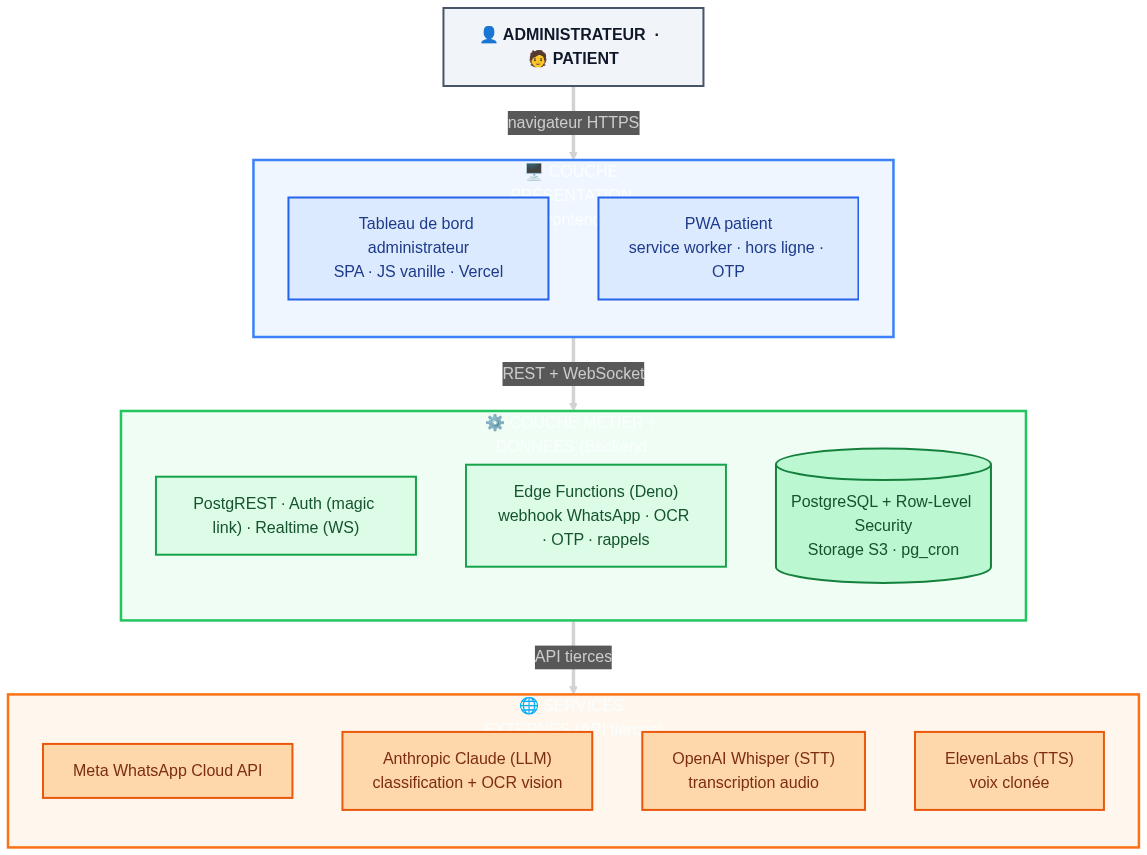
\includegraphics[width=.72\textwidth,height=1.0\textheight,keepaspectratio]{figures/nova-archi.png}%
}{%
  \fbox{\parbox[c][8cm][c]{0.42\textwidth}{\centering\itshape\small
    [Architecture globale (vue verticale) -- a generer depuis\\
    \texttt{figures/sources/nova-archi.mmd} via\\
    \url{https://mermaid.live} puis sauvegarder en\\
    \texttt{figures/nova-archi.png}]
  }}%
}
\caption{Architecture globale de \nova{} : trois couches empilées verticalement -- frontends, backend Supabase, services externes.}
\label{fig:nova-archi}
\end{figure}


Les sept composants sont : (1) le canal conversationnel WhatsApp Business
Cloud API, enregistre au numero de telephone de chaque locataire ; (2) le
recepteur de webhook (\texttt{whatsapp-webhook}), une fonction Edge
Supabase qui dispatche chaque message a la bonne entreprise ; (3) le
cerveau IA (\texttt{classify-message}), une seconde fonction Edge qui
encapsule Claude Haiku avec un prompt systeme produisant du JSON
structure ; (4) la couche de persistance, une base Postgres Supabase
avec Row-Level Security ; (5) le tableau de bord proprietaire, une
application monopage servie depuis Vercel ; (6) la PWA patient
(\texttt{/pwa/}), separee mais connectee au meme backend ; (7) la couche
de cron \texttt{pg\_cron} qui declenche les rappels, les campagnes de
remplissage de creneaux et les batchs d'anniversaire.

% =============================================================================
%  Methodologie du projet --- inchangee, traduite en francais
% =============================================================================
\section{Methodologie du projet}
La gestion de projet est une etape essentielle pour assurer la livraison
reussie d'une plateforme multi-locataire de receptionniste virtuelle.
Plusieurs methodologies de gestion de projet sont disponibles pour aider
les equipes a planifier, executer et adapter leur travail efficacement.
Parmi celles-ci, la methodologie Scrum est particulierement adaptee aux
projets qui combinent developpement d'IA conversationnelle, exigences
metier evolutives, et retours rapides des clients --- caracteristiques
qui definissent precisement le projet Nova~AI.

\subsection{La methode Scrum}
Scrum est aujourd'hui la methode Agile la plus populaire. L'approche Scrum
suit les principes du manifeste Agile, ce qui implique une participation
active du client tout au long du projet. Le terme \og scrum \fg{} provient
du vocabulaire sportif et designe la melee au rugby. Le principe de base
est que l'equipe avance comme une seule unite et reste prete a reorienter
le projet a mesure qu'il progresse, a l'image d'une melee ou les joueurs,
en groupe solidaire, s'adaptent collectivement au mouvement du ballon.

La methodologie Scrum repose sur des \emph{sprints}, qui sont des
intervalles de temps relativement courts, generalement de deux a quatre
semaines. A la fin de chaque sprint, l'equipe presente ce qu'elle a
ajoute au produit. La figure \ref{fig:scrum-cycle} resume le cycle de vie
d'un projet Scrum.

% ===========================================================================
% Cycle de vie d'un projet Scrum
% ===========================================================================
\begin{figure}[H]
\centering
\begin{tikzpicture}[
  font=\footnotesize,
  every node/.style={align=center},
  pb/.style    ={rectangle, rounded corners=2pt, draw=black!75,
                 fill=violet!15, minimum width=30mm, minimum height=14mm,
                 font=\scriptsize\bfseries},
  sb/.style    ={pb, fill=cyan!12, minimum width=30mm},
  ev/.style    ={pb, fill=orange!12, minimum width=24mm},
  artif/.style ={pb, fill=green!12, minimum width=24mm},
  arrow/.style ={->, thick, draw=black!75, >=Stealth},
  loop/.style  ={->, thick, draw=violet!70, >=Stealth, dashed},
]

% Linear flow left → right
\node[pb]    (pbacklog) at (0, 0) {Product\\Backlog};
\node[ev]    (planning) at (3.6, 0) {Sprint\\Planning};
\node[sb]    (sbacklog) at (7.0, 0) {Sprint\\Backlog};

% Sprint loop (in the middle)
\node[ev]    (daily) at (10.5, 1.6) {Daily\\Scrum};
\node[artif] (incr)  at (10.5, 0)   {Incrément};
\node[ev]    (review)at (10.5,-1.6) {Sprint\\Review};

% Final
\node[ev]    (retro) at (14.5, 0) {Sprint\\Retrospective};

% Linear arrows
\draw[arrow] (pbacklog) -- (planning);
\draw[arrow] (planning) -- (sbacklog);
\draw[arrow] (sbacklog) -- ++(2.0,0) |- (daily.west);

% Sprint inner cycle (24h loop daily-incrément-daily)
\draw[loop] (daily.south)  -- (incr.north);
\draw[loop] (incr.south)   -- (review.north);
\draw[loop] (review.west)  to[bend left=45]
   node[midway, fill=white, font=\scriptsize, inner sep=1pt]{2--4 sem.}
   (daily.west);

% From review/retrospective back to product backlog (refinement)
\draw[arrow] (incr.east)  -- (retro.west);
\draw[arrow] (retro.north) to[bend right=30]
   node[midway, fill=white, font=\scriptsize, inner sep=1pt]{nouveau sprint}
   (pbacklog.north);

% Caption notes
\node[font=\scriptsize\itshape, below=14mm of pbacklog, anchor=north, xshift=0mm] (legend1) {priorisé par le Product Owner};
\node[font=\scriptsize\itshape, below=14mm of sbacklog, anchor=north] (legend2) {engagement de l'équipe};
\node[font=\scriptsize\itshape, below=14mm of incr, anchor=north] (legend3) {potentiellement livrable};
\node[font=\scriptsize\itshape, below=14mm of retro, anchor=north] (legend4) {amélioration continue};

\end{tikzpicture}
\caption{Cycle de vie d'un projet Scrum : un Product Backlog priorisé alimente chaque Sprint Planning ; le Sprint Backlog devient l'engagement de l'équipe pour 2 à 4 semaines, rythmé par des Daily Scrums quotidiens, et clôturé par une Sprint Review (démo) et une Sprint Retrospective (amélioration continue).}
\label{fig:scrum-cycle}
\end{figure}


Pour le projet Nova~AI, nous avons structure notre processus Scrum afin
de prendre en compte trois flux de travail entrelaces : le developpement
back-end sur Supabase (schema de base de donnees, fonctions Edge,
souscriptions temps reel), le travail front-end sur le tableau de bord
multi-locataire et la PWA patient, et l'ingenierie de prompts pour le
receptionniste IA qui gere les conversations WhatsApp en arabe, francais
et anglais.

\subsubsection{Roles Scrum}
\begin{itemize}
  \item \textbf{L'equipe.} Responsable de transformer les exigences
        definies par le Product Owner en fonctionnalites utilisables.
        Dans notre projet, l'equipe est full-stack et combine ingenierie
        front-end sur le tableau de bord, ingenierie back-end sur Postgres
        et les fonctions Edge Deno, ingenierie IA pour le classifieur
        d'intention base sur Claude et le verificateur de securite des
        prescriptions, ainsi que conception UI/UX pour la page d'accueil
        au theme \emph{anti-gravite} et l'interface de la PWA.
  \item \textbf{Le Scrum Master.} Responsable de la comprehension, du
        respect et de l'organisation de la methodologie Scrum. Il garantit
        que les iterations de prompts IA, les migrations de schema et les
        evolutions du tableau de bord progressent harmonieusement et
        conformement aux principes de Scrum, en levant les obstacles tels
        que les delais de verification de l'API Meta WhatsApp ou les
        contraintes de quota d'ElevenLabs.
  \item \textbf{Le Product Owner.} Represente generalement le client et
        porte la vision du produit a creer. Pour notre projet, le role de
        Product Owner agrege les perspectives de trois personae cibles :
        un proprietaire de clinique tunisien, un responsable de
        laboratoire d'analyses, et un medecin independant. Leurs points
        de douleur recurrents (rendez-vous manques, prescriptions
        manuscrites, prises de rendez-vous hors heures) ont oriente la
        priorisation du Product Backlog.
\end{itemize}

\subsubsection{Evenements Scrum}
\begin{itemize}
  \item \textbf{Sprint Planning.} Les taches a accomplir durant le sprint
        sont determinees par l'ensemble de l'equipe Scrum lors de la
        reunion de planification. Pour Nova~AI, cette planification couvre
        a la fois le travail produit (un nouvel onglet du tableau de bord,
        une migration Postgres, un gestionnaire de reponse a un bouton
        WhatsApp) et le travail IA (raffinement de la machine d'etats de
        prise de rendez-vous, extension du prompt de securite des
        medicaments).
  \item \textbf{Sprint Review.} Il s'agit de l'evaluation du sprint
        accompli. Une fois le sprint termine, l'equipe et les parties
        prenantes se reunissent pour valider ce qui a ete realise. Pour
        notre projet, cela inclut la demonstration des nouveaux onglets du
        tableau de bord, l'execution d'un parcours de prise de rendez-vous
        de bout en bout sur un vrai numero Meta, et la revue des
        transcriptions de l'IA sur les cas limites.
  \item \textbf{Sprint Retrospective.} Vise a s'adapter aux changements et
        a ameliorer continuellement le processus de mise en oeuvre.
        L'equipe utilise la retrospective pour examiner le sprint termine
        et determiner ce qui a bien fonctionne et ce qui doit etre
        ameliore. Cette pratique a ete particulierement precieuse pour
        affiner la strategie de prompt IA apres avoir observe des
        mauvaises classifications en conditions reelles, et pour
        renforcer les politiques de Row-Level Security multi-locataire
        apres chaque nouvelle fonctionnalite.
  \item \textbf{Daily Scrum.} Cette reunion quotidienne de quinze minutes
        est tres importante. Son objet est de suivre la progression
        quotidienne du sprint. Pour notre projet, le stand-up quotidien
        couvre l'avancement des composants du tableau de bord, des
        deploiements de fonctions Edge, des revisions de prompts IA et
        des tests de migrations Supabase.
\end{itemize}

\subsubsection{Artefacts Scrum}
\begin{itemize}
  \item \textbf{Le Product Backlog.} Une liste priorisee des exigences
        initiales du client pour le produit a creer. Le Product Owner est
        responsable du Product Backlog. Notre Product Backlog couvre les
        user stories pour la prise de rendez-vous, les rappels, le
        pipeline de laboratoire, le remplissage de creneaux a la demande,
        l'apprentissage des durees de consultation, la securite des
        medicaments, les profils de vehicules, les surprises
        d'anniversaire, le check-in QR, la file d'attente en temps reel,
        et l'application web progressive pour les patients.
  \item \textbf{Le Sprint Backlog.} Le plan detaille pour atteindre
        l'objectif du sprint, defini lors de la reunion de planification.
        Pour notre projet, chaque Sprint Backlog contenait un melange de
        migrations de base de donnees, de taches de fonctions Edge, de
        travaux d'IHM et d'experiences d'ingenierie de prompts ---
        typiquement de trois a six user stories dimensionnees pour tenir
        dans un sprint de deux semaines.
\end{itemize}

\subsection{Justification du choix de la methodologie Agile Scrum}
La methodologie Agile Scrum est particulierement adaptee au projet
Nova~AI en raison de sa flexibilite intrinseque et de sa nature
iterative, qui s'alignent bien avec les exigences evolutives d'une
plateforme IA multi-locataire desservant des entreprises heterogenes
(cliniques, laboratoires, salons, garages, medecins independants).
Comme le systeme inclut des fonctionnalites avancees telles qu'un
receptionniste IA multi-tour, une messagerie WhatsApp en temps reel,
une OCR de prescriptions par modele de vision, des durees de
consultation auto-apprises, du remplissage de creneaux a la demande,
et une file d'attente en temps reel, Scrum a permis a l'equipe de
livrer des increments fonctionnels de maniere fiable tout en
accommodant les priorites changeantes.

L'accent mis par la methodologie sur la collaboration trans-fonctionnelle
a favorise une integration sans heurts entre la logique front-end
(l'IHM du tableau de bord au theme anti-gravite), les services back-end
(Postgres Supabase, fonctions Edge, Storage, Realtime) et les composants
IA (Claude Haiku pour la classification d'intention, Claude Sonnet pour
l'OCR des images de prescriptions, ElevenLabs en option pour le clonage
vocal). De plus, son cadre ouvert avec des stand-ups quotidiens et des
sprint reviews garantit que les parties prenantes restent engagees tout
au long du processus de developpement.

La methodologie a ete particulierement precieuse en cela qu'au fur et a
mesure que le projet s'est etendu pour englober de nouveaux types
d'entreprises et de nouvelles capacites --- profils de vehicules pour
garages, gestion de file d'attente pour laboratoires, verificateur
d'interactions medicamenteuses --- elle a soutenu une amelioration
continue basee sur les retours utilisateurs reels et sur l'evolution
des besoins du marche dans le contexte tunisien.

Cette methode a ete tres benefique pour notre projet, car elle nous a
permis de mettre en oeuvre efficacement la prise de rendez-vous assistee
par IA, la gestion temps reel des rendez-vous, et les flux metiers
intelligents pour les petites et moyennes entreprises tunisiennes, tout
en restant centre sur les objectifs metier et en adressant les defis
techniques d'un developpement SaaS multi-locataire.


\section{Conclusion}
Ce chapitre a pose le decor : nous a